\documentclass{beamer}

\usepackage[utf8]{inputenc}
\usepackage[brazilian]{babel}
\usepackage{graphicx}
\usepackage{subcaption}
\usepackage{listings}

\title{Visão Computacional e Aprendizado de Máquina}
\subtitle{Breve introdução}
\author{Vitor Greati\inst{1} \and Vinícius Campos\inst{1}}
\institute[]
{
	\inst{1}%
	Universidade Federal do Rio Grande do Norte
}
\date{}
\subject{Computer Science}

% Table of contents at the beginning of each section
\AtBeginSection[]
{
  \begin{frame}
    \frametitle{Sumário}
    \tableofcontents[currentsection, currentsubsection]
  \end{frame}
}

% Table of contents at the beginning of each subsection
%\AtBeginSubsection[]
%{
%  \begin{frame}
%    \frametitle{Table of Contents}
%    \tableofcontents[currentsection,currentsubsection]
%  \end{frame}
%}

\begin{document}

\frame{\titlepage}

\section{O gap semântico}

    \begin{frame}{O que você percebe nestas imagem?}

        \begin{figure}
            \centering
            \begin{subfigure}[b]{0.5\textwidth}
                \centering
                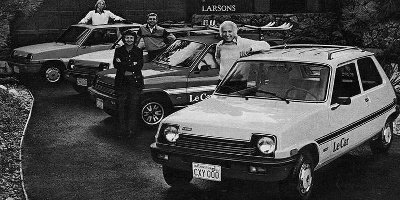
\includegraphics[height=2.6cm]{img/gcarpeople.jpg}
                \label{fig:carpeople}
            \end{subfigure}~
            \begin{subfigure}[b]{0.5\textwidth}
                \centering
                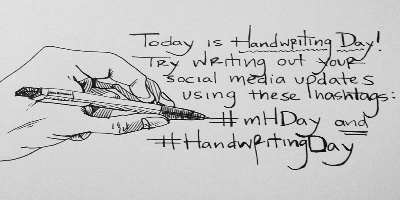
\includegraphics[height=2.6cm]{img/ghandwriting.jpg}
                \label{fig:handwriting}
            \end{subfigure}

            \begin{subfigure}[b]{0.5\textwidth}
                \centering
                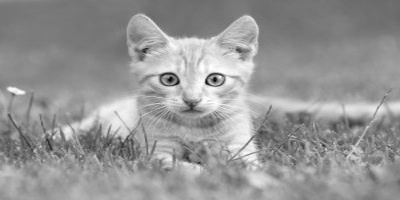
\includegraphics[height=2.6cm]{img/gcat.jpg}
                \label{fig:carpeople}
            \end{subfigure}~
            \begin{subfigure}[b]{0.5\textwidth}
                \centering
                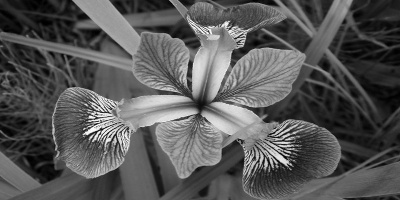
\includegraphics[height=2.6cm]{img/giris.jpg}
                \label{fig:handwriting}
            \end{subfigure}
        \end{figure}

        \pause

        A facilidade com que respondemos a essa pergunta
        se deve ao nosso sistema visual \textbf{nativo} 
        extremamente
        poderoso!

    \end{frame}

    \begin{frame}[fragile]{O que o computador percebe nessas imagens}{As matrizes de \emph{pixels}}

        À primeira vista\ldots

        \begin{columns}
            \begin{column}{0.4\textwidth}
        {\tiny
            %cars
        \begin{lstlisting}
[[ 42  23  19 ...,  21  29  25]
 [ 40  40  36 ...,  24  24  21]
 [ 28  30  36 ...,  30  13  27]
 ...,
 [115  78  45 ...,  28  36  17]
 [ 67  78 192 ...,  35  31  36]
 [ 67  79 104 ...,  34  32  31]]
        \end{lstlisting}}

        {\tiny
            % cat
        \begin{lstlisting}
[[138 137 137 ..., 107 107 107]
 [135 134 134 ..., 107 107 107]
 [130 129 129 ..., 107 107 107]
 ..., 
 [145 145 146 ..., 142 142 142]
 [146 145 144 ..., 144 144 145]
 [147 146 144 ..., 145 145 146]]
        \end{lstlisting}}
            \end{column}
            \begin{column}{0.5\textwidth}

        {\tiny
            % hand
        \begin{lstlisting}
[[222 224 224 ..., 204 201 200]
 [223 225 223 ..., 201 203 204]
 [226 226 226 ..., 204 202 205]
 ..., 
 [210 203 208 ..., 192 188 189]
 [206 206 207 ..., 190 188 189]
 [210 208 210 ..., 191 193 185]]
        \end{lstlisting}}

        {\tiny
            % iris
        \begin{lstlisting}
[[ 48  45  40 ...,  28  29  31]
 [ 45  46  43 ...,  28  29  30]
 [ 41  43  43 ...,  27  27  29]
 ..., 
 [101 101 103 ...,  64  51  32]
 [ 98  97  99 ...,  63  71  57]
 [ 97  97  97 ...,  38  57  65]]
        \end{lstlisting}}

            \end{column}
        \end{columns}

        \pause

        \begin{block}{Imagens digitais monocromáticas}
            Matrizes $I_j \in \mathbb{M}_{w_j \times h_j}([0,\ldots,255])$
 ou funções $f_j:\{1,\ldots,w_j\} \times \{1,\ldots,h_j\} 
 \to [0,255]$, onde $w_j$ é a largura e $h_j$ é a altura da imagem $j$.
        \end{block}

    \end{frame}
    
    \begin{frame}{O \emph{gap} semântico}{Percepção humana $\times$ Percepção da máquina}

        \begin{block}{\emph{Gap} semântico}
            Diferença entre a maneira como o ser humano \textbf{percebe} o conteúdo de uma imagem
            e como a imagem pode ser \textbf{representada} de forma manipulável no computador.
        \end{block}
    
    \end{frame}

\section{Visão Computacional}

    \subsection{Para além de \emph{pixels}}

    \begin{frame}{Visão Computacional}{O que é?}

        \begin{block}{Visão Computacional}
        Visão Computacional é uma área da Ciência da Computação
        cujo propósito é capacitar os computadores para extraírem
        informações de imagens, ou seja, permitir que tenham
        um entendimento visual do mundo.
        \end{block}

        \pause

        Algumas das práticas mais comuns 
        estão ligadas à tarefa de \textbf{reconhecimento}, nas formas de:
        \pause
        \begin{itemize}
            \item<1-> Classificação de objetos
            \item<2-> Identificação
            \item<3-> Detecção
        \end{itemize}

    \end{frame}

    \begin{frame}{Visão Computacional}{Desafios}
        
        \begin{alertblock}{Variação de ponto de vista}
            Não importa sob qual ângulo se fotografe um gato:
            ele continuará sendo um gato.
        \end{alertblock}

        \begin{alertblock}{Variação de escala}
            Não importa a que distância o gato estará da câmera:
            ele continuará sendo um gato.
        \end{alertblock}

        \begin{alertblock}{Deformação}
            Um gato pode estar esticando suas pernas ou/e contorcendo
            seu pescoço para se lamber, e isso não o faz ser
            outro ser além de um gato na imagem.
        \end{alertblock}

    \end{frame}

    \begin{frame}{Visão Computacional}{Desafios}

        \begin{alertblock}{Oclusão}
            Um gato pode estar espiando o mundo ao redor de dentro de uma
            caixa, apenas com a cabeça de fora, e ele continuará sendo um gato à lente de uma câmera
            em frente à caixa.
        \end{alertblock}

        \begin{alertblock}{Iluminação}
            Um gato num estacionamento mal iluminado ainda é um gato.
        \end{alertblock}

        \begin{alertblock}{Ruído de fundo}
            Um gato em frente à uma tela de TV repleta de ruído
            ainda é um gato.
        \end{alertblock}

        \begin{alertblock}{Variações intra-classe}
            Gatos de diversas raças, cores e tamanhos serão
            sempre gatos.
        \end{alertblock}
    \end{frame}

    \subsection{Aplicações}
    \begin{frame}{Aplicações}{Reconhecimento Automático de Placas}

\begin{figure}
    \centering
    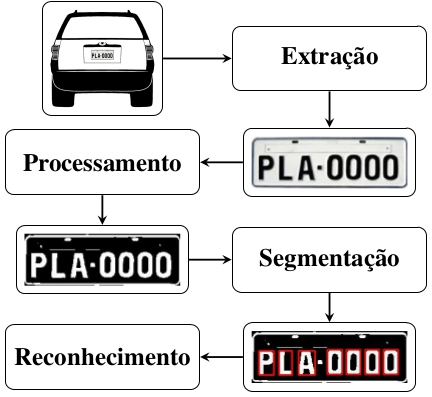
\includegraphics[scale=.4]{img/lpr.jpeg}
    \caption{Etapas gerais de um processo de RAP. (Fonte: Autoral)}
    \label{fig:lpr_recognition}
\end{figure}

\end{frame}

\begin{frame}{Aplicações}{Reconhecimento de Faces (Expressões)}

\begin{figure}
    \centering
    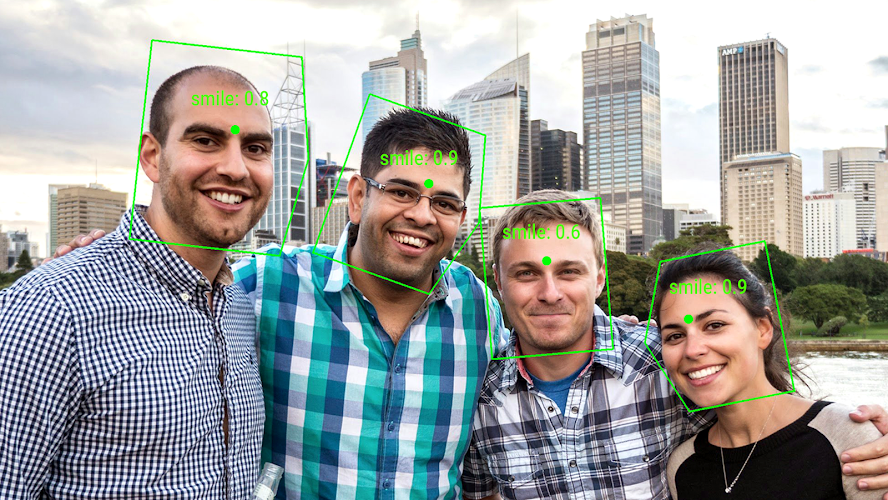
\includegraphics[scale=.3]{img/face_recognition.png}
    \caption{Reconhecimento de faces e de expressões. (Fonte: Mobile Vision - https://developers.google.com/vision/)}
    \label{fig:face_recognition}
\end{figure}

\end{frame}

\begin{frame}{Aplicações}{Reconhecimento de gestos}

\begin{figure}
    \centering
    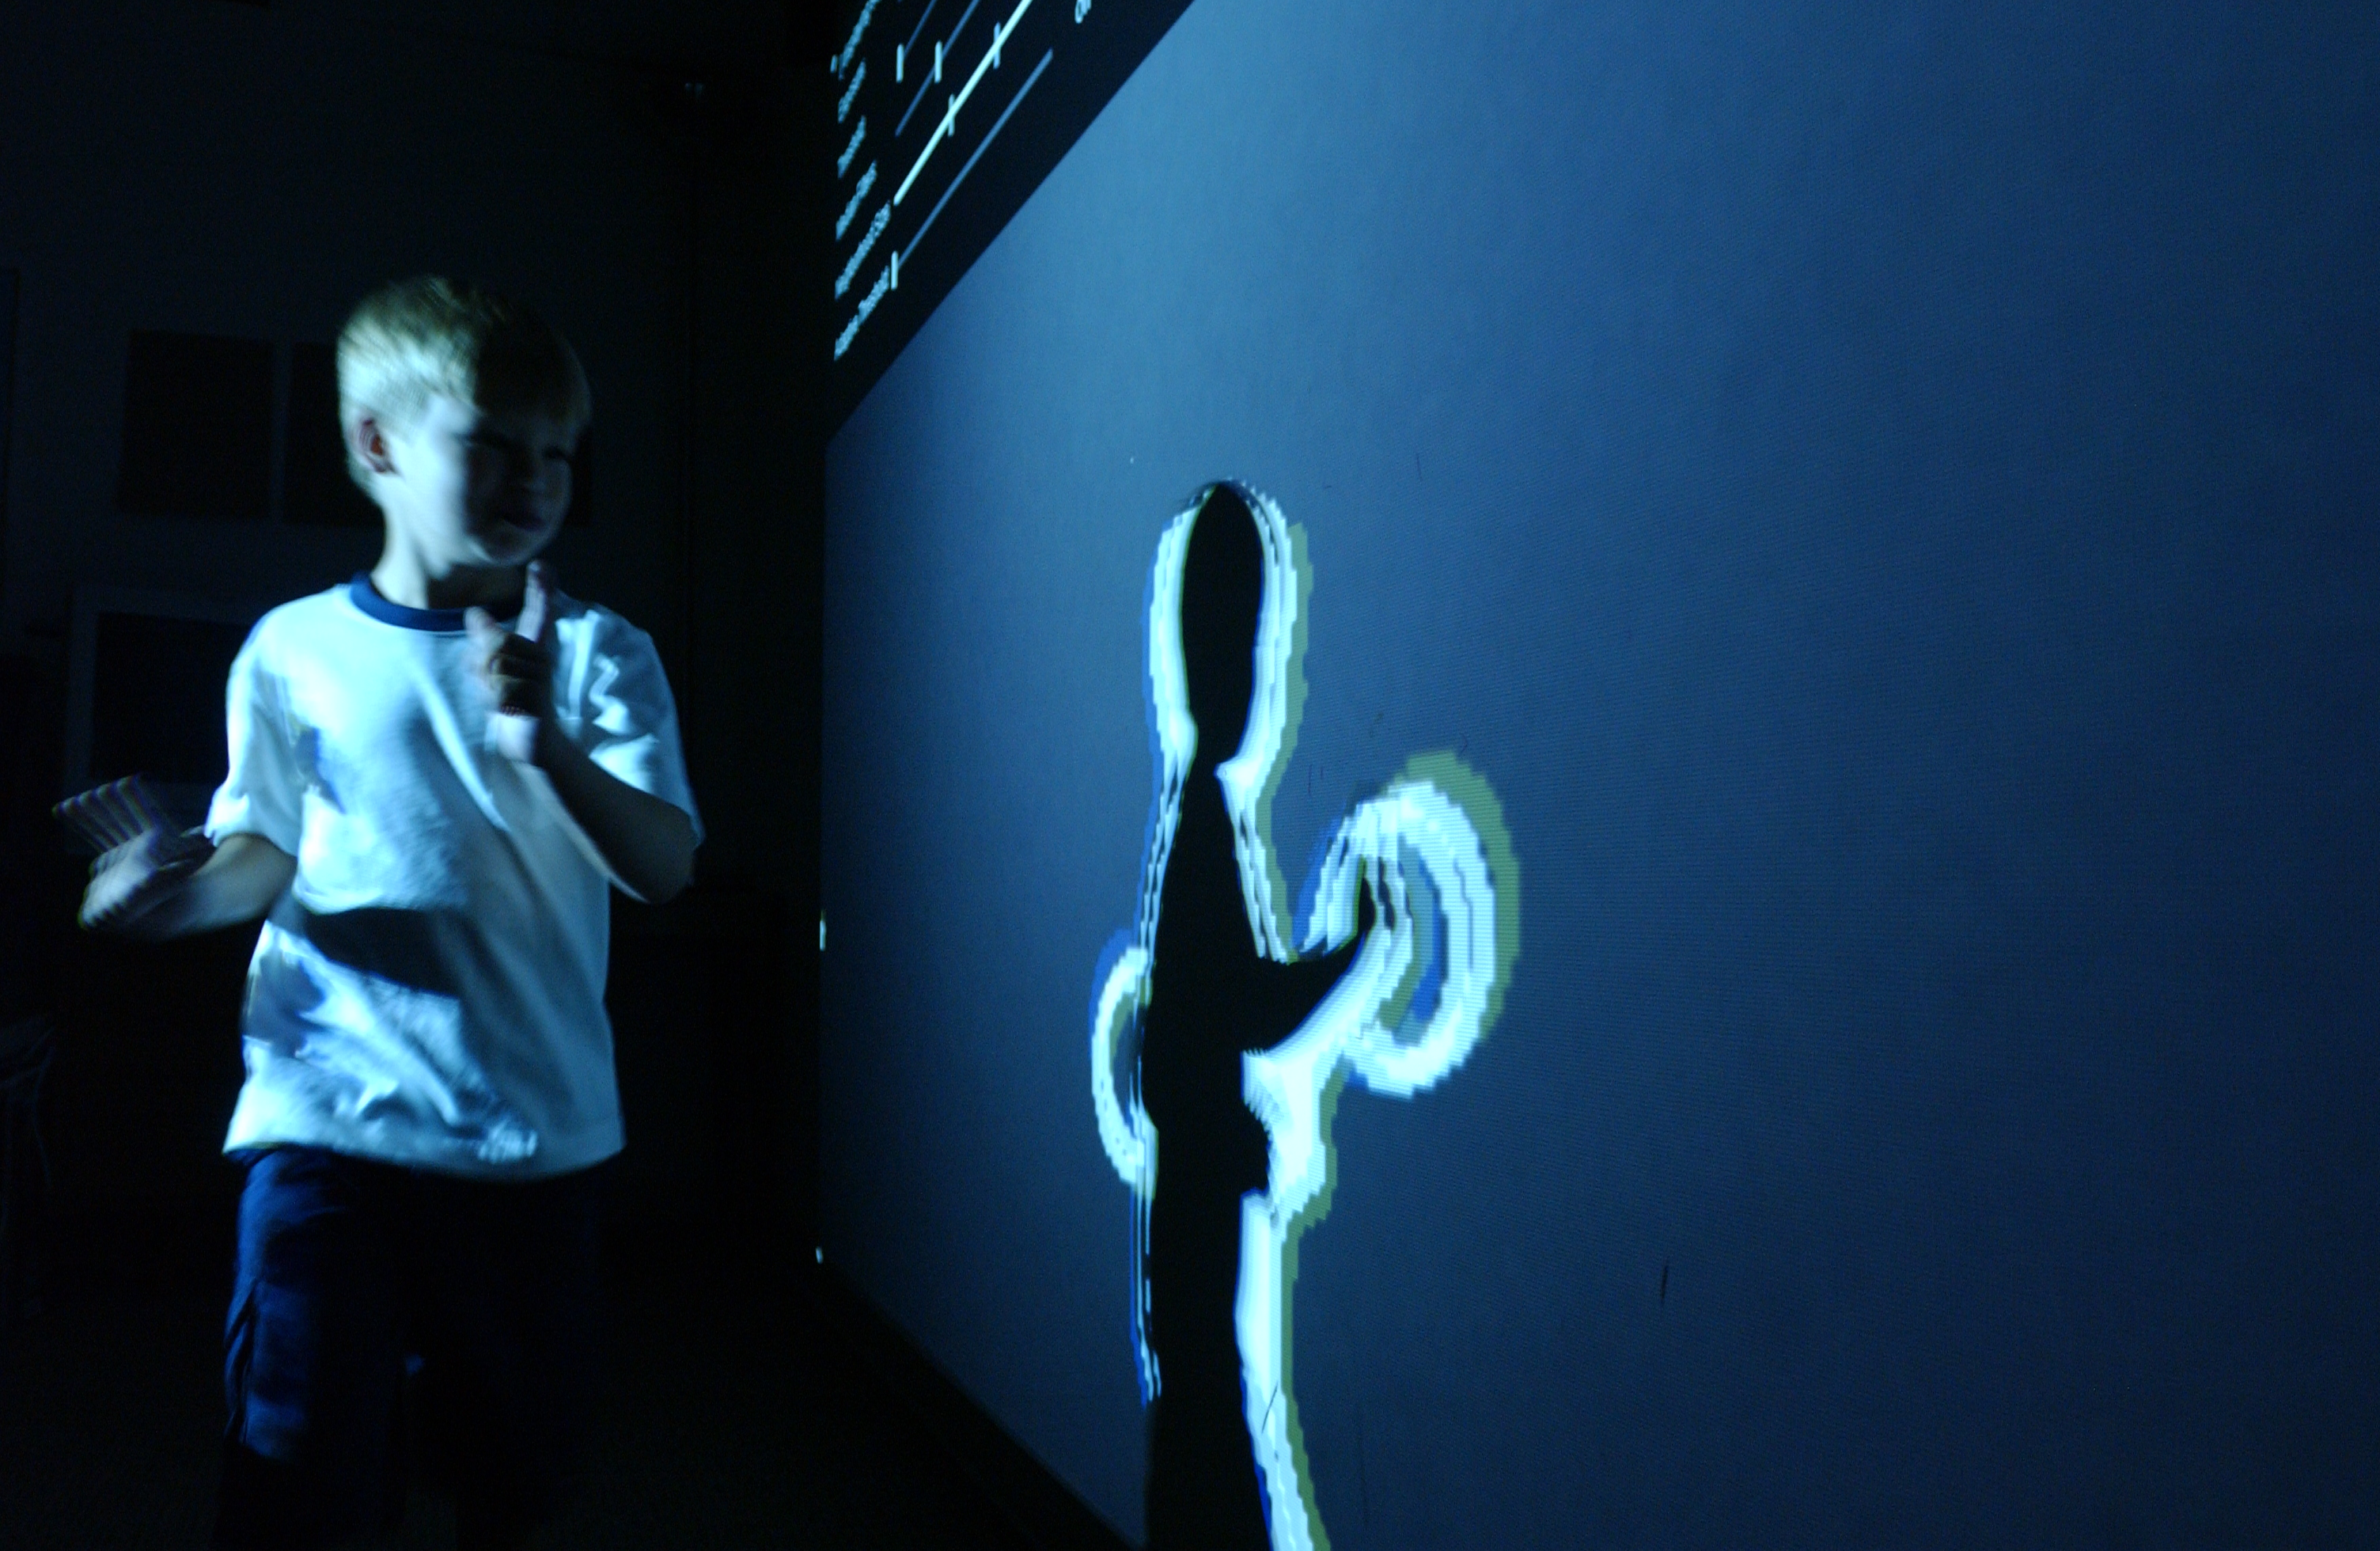
\includegraphics[scale=.4]{img/gesture_recognition.jpg}
    \caption{(Fonte: Wikipedia - https://en.wikipedia.org/ \\ wiki/Gesture\_recognition)}
    \label{fig:gesture_recognition}
\end{figure}

\end{frame}

\begin{frame}{Aplicações}{Veículos Autônomos}

\begin{figure}
    \centering
    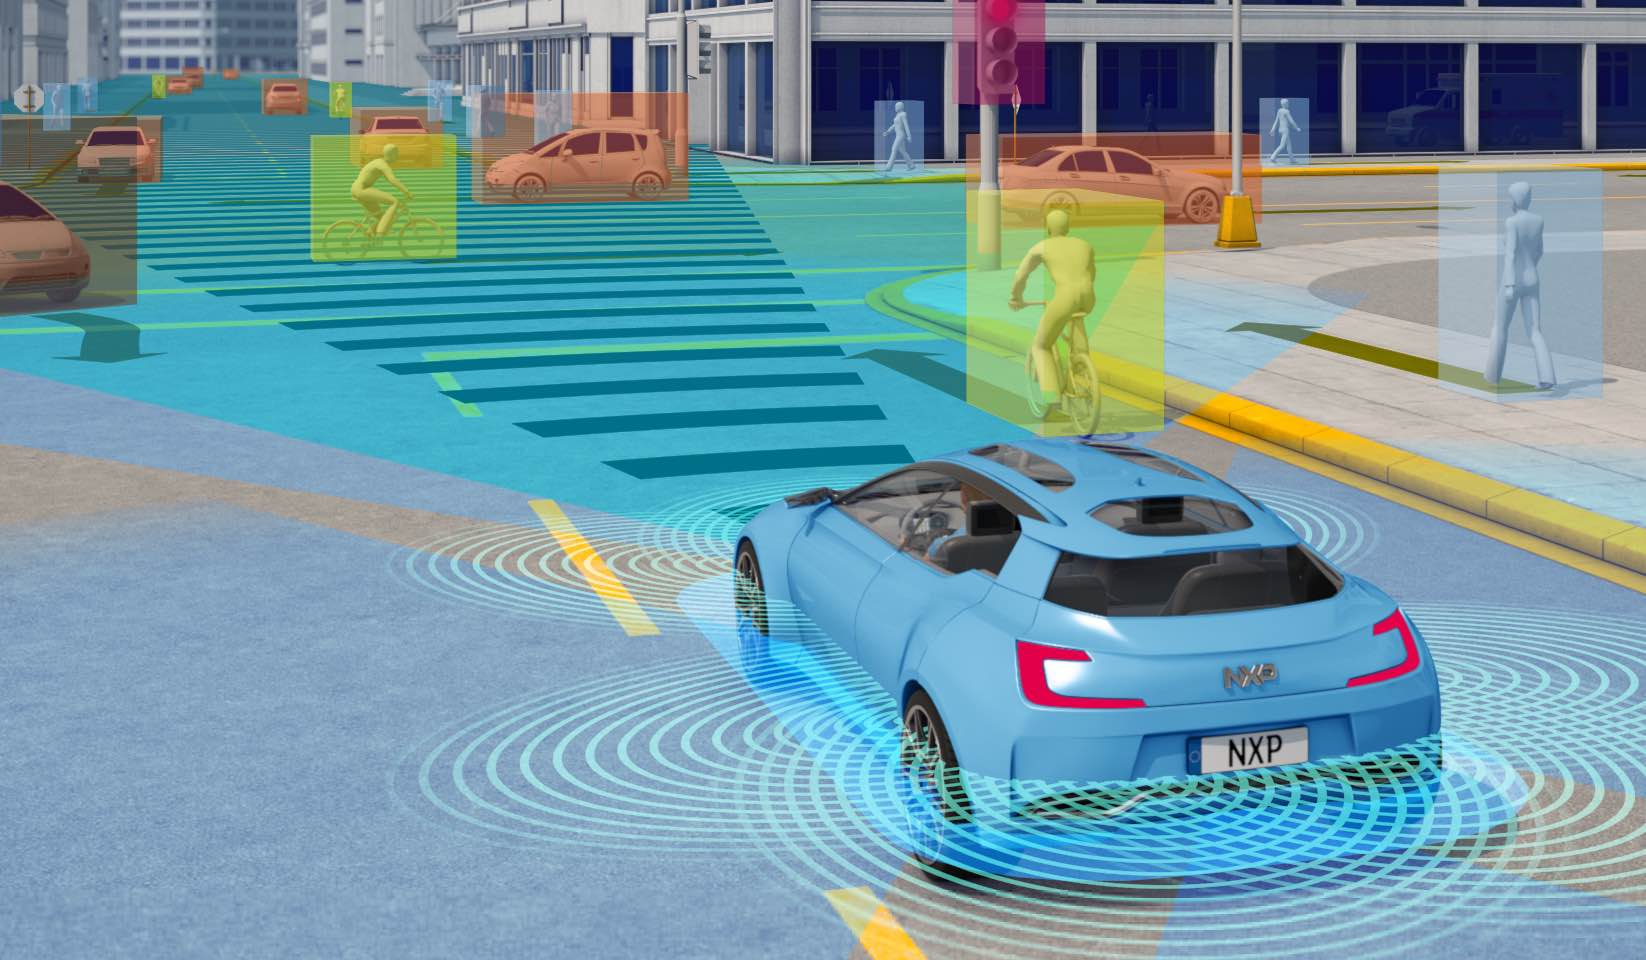
\includegraphics[scale=.18]{img/autonomous_car.jpg}
    \caption{(Fonte: Electronics Weekly - https://www.electronicsweekly.com/market-sectors/automotive-electronics/ces-autonomous-cars-sensors-make-safe-2017-01/)}
    \label{fig:gesture_recognition}
\end{figure}

\end{frame}

\begin{frame}{Aplicações}{Coleções de Fotos Pessoais}

\begin{figure}
    \centering
    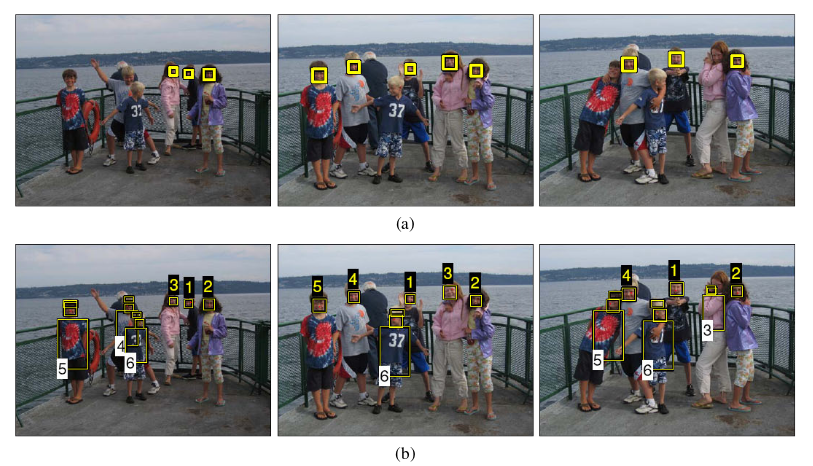
\includegraphics[scale=.3]{img/personal_collection.png}
    \caption{(Fonte: Computer Vision - Algorithms and Applications - Richard Szeliski)}
    \label{fig:personal_collection}
\end{figure}

\end{frame}

\begin{frame}{Aplicações}{Reconhecimento de Locais}

\begin{figure}
    \centering
    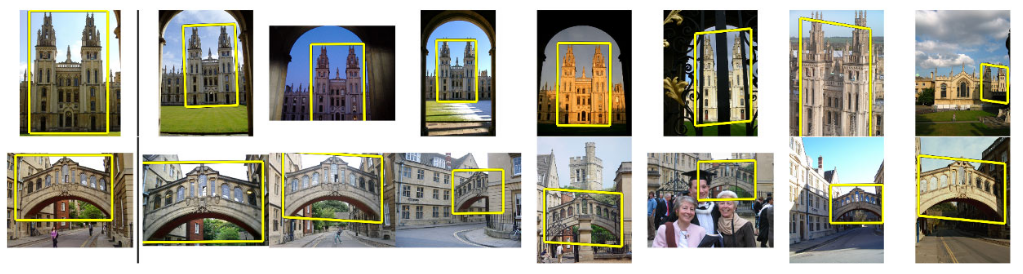
\includegraphics[scale=.3]{img/location_recognition.png}
    \caption{(Fonte: Computer Vision - Algorithms and Applications - Richard Szeliski)}
    \label{fig:location_recognition}
\end{figure}

\end{frame}

\begin{frame}{Aplicações}{Edições Inteligentes}

\begin{figure}
    \centering
    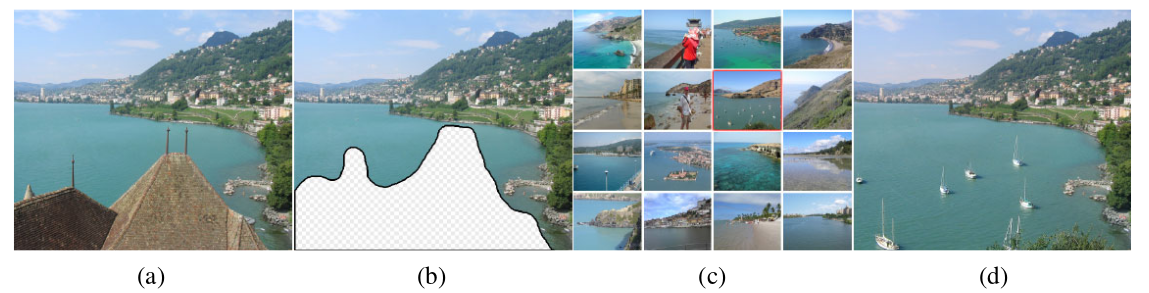
\includegraphics[scale=.28]{img/smart_editing.png}
    \caption{(Fonte: Computer Vision - Algorithms and Applications - Richard Szeliski)}
    \label{fig:smart_editing}
\end{figure}

\end{frame}

\begin{frame}{Aplicações}{Segmentação de Imagens Médicas}

\begin{figure}
    \centering
    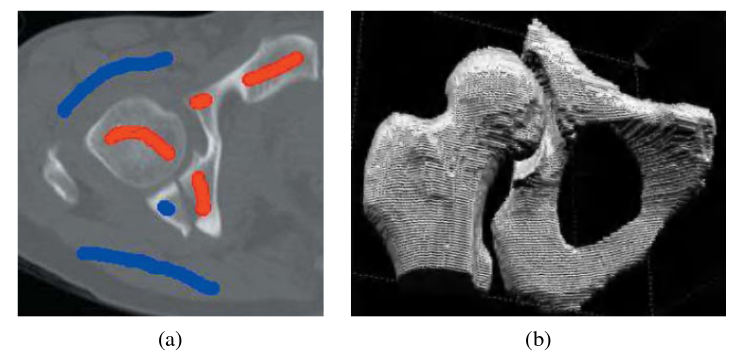
\includegraphics[scale=.4]{img/medical_image_segmentation.png}
    \caption{(Fonte: Computer Vision - Algorithms and Applications - Richard Szeliski)}
    \label{fig:medical_image_segmentation}
\end{figure}

\end{frame}

\begin{frame}{Aplicações}{Rastreamento de Contorno e Rotoscopia}

\begin{figure}
    \centering
    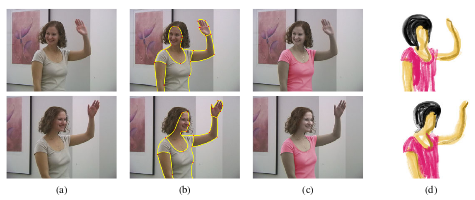
\includegraphics[scale=.6]{img/contour_trackin_rotoscoping.png}
    \caption{(Fonte: Computer Vision - Algorithms and Applications - Richard Szeliski)}
    \label{fig:contour_tracking_rotoscoping}
\end{figure}

\end{frame}

\begin{frame}{Aplicações}{Reconhecimento Ótico de Braille}

\begin{figure}
    \centering
    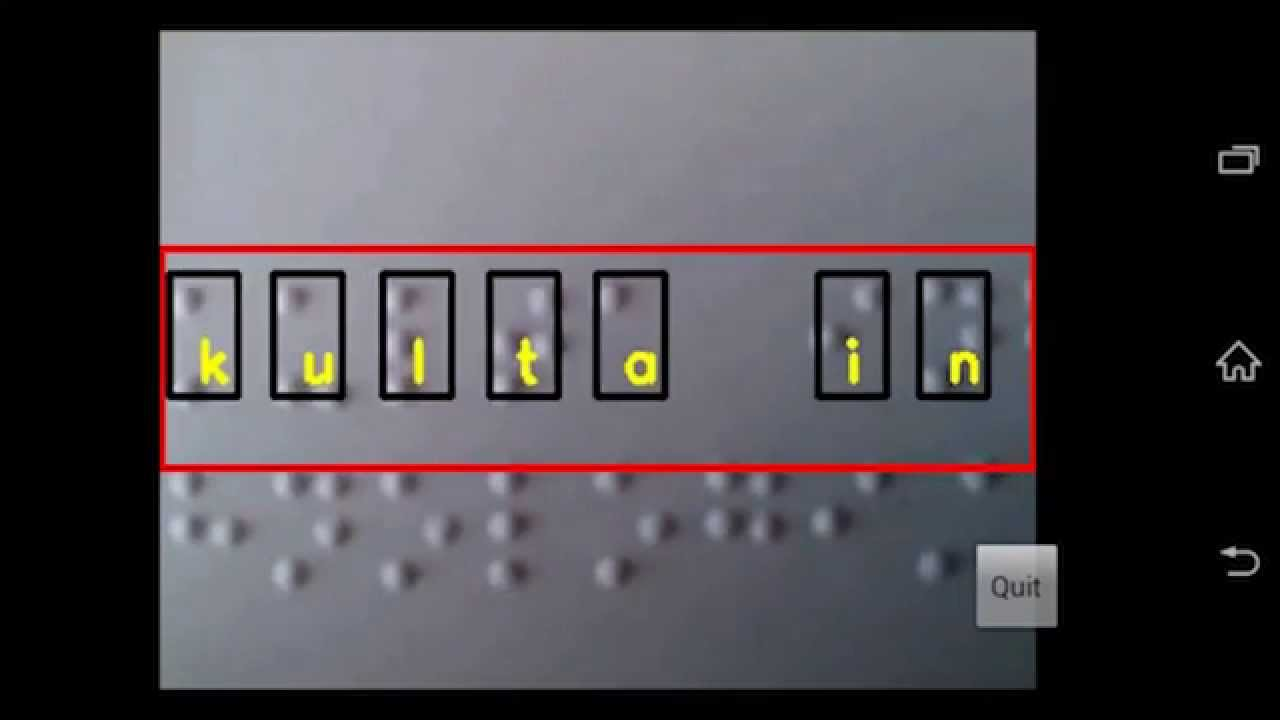
\includegraphics[scale=.2]{img/obr.jpg}
    \caption{(Fonte: Youtube - https://www.youtube.com/watch?v=X5kFdUsCkEA)}
    \label{fig:optical_braille_recognition}
\end{figure}

\end{frame}

\begin{frame}{Aplicações}{Reconhecimento de Impressões Digitais}

\begin{figure}

    \centering
    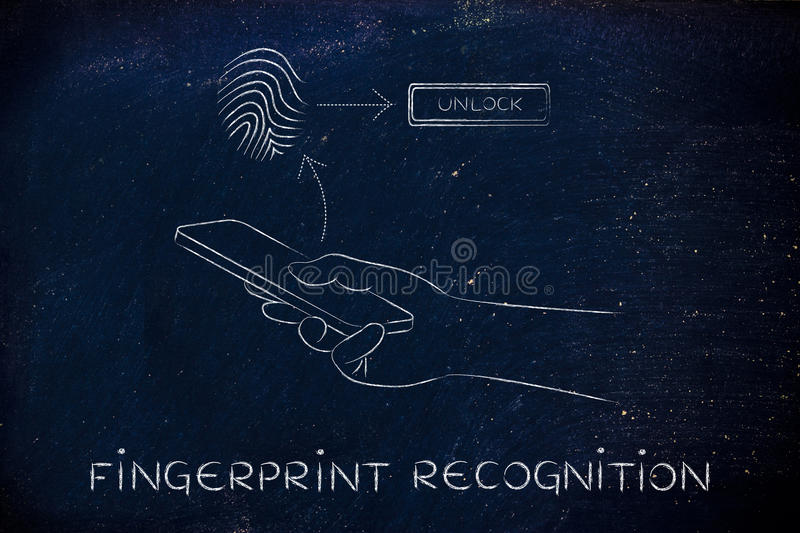
\includegraphics[scale=1]{img/fingerprint_recognition.jpg}
    \caption{(Fonte: Dreamstime - https://thumbs.dreamstime.com/b/fingerprint-recognition-smartphones-smartphone-user-touching-screen-to-unlock-68633965.jpg)}
    \label{fig:fingerprint_recognition}
\end{figure}

\end{frame} 

\begin{frame}{Aplicações}{Reconhecimento de Iris}

\begin{figure}

    \centering
    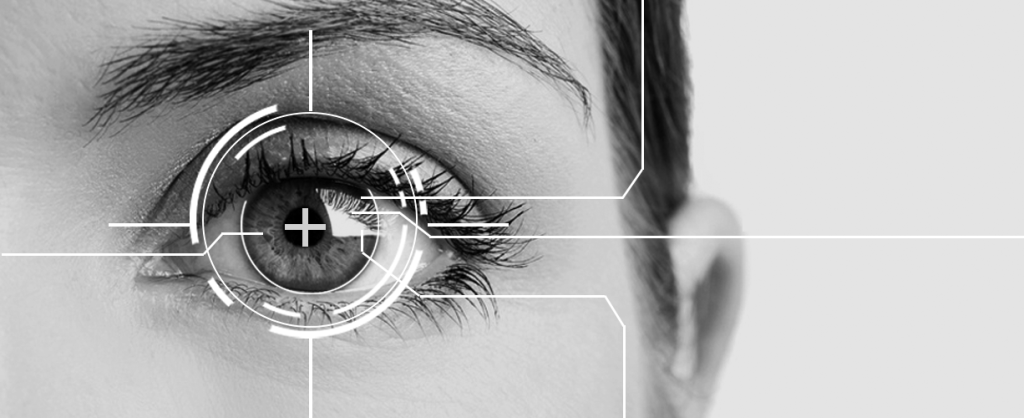
\includegraphics[scale=.3]{img/iris_recognition.png}
    \caption{(Fonte: Iritech - http://www.iritech.com/blog/iris-biometric-safe/)}
    \label{fig:iris_recognition}
\end{figure}

\end{frame}


    \subsection{Técnicas}

\section{Aprendizagem de Máquina}


\end{document}
